\documentclass[10pt,a4paper]{article}
\usepackage[utf8]{inputenc}
\usepackage[T1]{fontenc}
\usepackage{amsmath,amssymb}
\usepackage[margin=1.7cm,top=1.5cm,bottom=1.5cm]{geometry}
\usepackage{lmodern,microtype,booktabs,array,enumitem,xcolor,hyperref,graphicx,float,pdflscape}
\hypersetup{colorlinks=true,urlcolor=blue!50!black,linkcolor=black}
\setlist{nosep,leftmargin=1.2em}
\setlength{\parindent}{0pt}\setlength{\parskip}{2.5pt}
\renewcommand{\arraystretch}{1.08}
\newcommand{\q}[1]{\par\smallskip\textbf{#1}\ }
\newcommand{\code}[1]{\texttt{\small #1}}
\begin{document}

{\large\textbf{Lab 2 · Lakehouse end-to-end en AWS: batch y streaming}}\hfill\small SI7006 · Grandes Datos\\
\small Andrés Vélez Rendón · Santiago Vélez Blandón · Eduardo Andrés Piñeros Manjarrés \hfill 6 de noviembre de 2026
\hrule\smallskip

\section*{1. Qué se construyó y cómo se ejecutó}
Se completaron los TODO de \code{ingest.py}, \code{producer.py}, los cinco jobs (\code{bronze}, \code{silver}, \code{gold}, \code{audit}, \code{stream}), \code{athena.sql} y \code{serverless.yml}. Todo se desarrolló y validó primero en local (Docker + Spark 3.5 + Delta 3.2 + Kafka) y luego se desplegó en AWS Academy Learner Lab (S3, Glue 5.0, Kinesis, Athena). El diagrama de la arquitectura está en \code{informe/diagrama/} (\code{.drawio}, \code{.pdf}, \code{.png}).

\begin{center}\small
\begin{tabular}{@{}p{4.1cm}p{6.6cm}p{5.2cm}@{}}\toprule
\textbf{Prueba} & \textbf{Local} & \textbf{AWS}\\\midrule
\code{pytest} & 15/15 en verde & ---\\
Lote 1 (2026-09-29) & validaciones \checkmark; 2.ª ejecución: 0 insertadas, 0 actualizadas & 4 jobs de Glue \emph{Succeeded}\\
Lote 2 (2026-09-30) & \checkmark; 1.ª: 1\,883 insertadas, 276 actualizadas; 2.ª: 0 y 0 & 4 jobs \emph{Succeeded}\\
Stream \emph{availableNow} & 12\,310 eventos; 2.ª ejecución: 0 filas leídas, tablas sin cambios & ---\\
Stream en vivo & 4\,858 filas en 180 s, validaciones \checkmark & \code{paytrack-stream} \emph{Succeeded} (9\,792 eventos, 109 ventanas, 89 alertas)\\
Athena & 6 consultas probadas con Spark SQL & 6 consultas ejecutadas (§4)\\\bottomrule
\end{tabular}
\end{center}

\textbf{Incidencias.} (i) Learner Lab no permite crear roles de IAM: \code{serverless.yml} usa el \code{LabRole} existente. (ii) El conector de Kinesis de Glue 5.0 entrega la hora de llegada en la columna \code{\$add\$record\_timestamp\$\_temporary\$} y no en \code{\_\_src\_timestamp}; \code{read\_events} (en \code{common.py}, archivo dado) fallaba con \code{KeyError}. Se diagnosticó imprimiendo \code{df.dtypes} en una ejecución corta y se corrigió aceptando ambos nombres (dos corridas \emph{Failed} previas en el historial de Glue).

\section*{2. Parte A · Batch}
\q{1. Bronze.} Lee todo como texto (\code{primitivesAsString}) porque el tipado es responsabilidad de Silver: un lote con un tipo distinto (p.\,ej. montos como \code{"40380.23"}, 600 de 30\,600 filas del lote 1) no rompe la tabla ni pierde el dato original. \code{replaceWhere} sobre \code{ingest\_date} reemplaza solo la partición del lote; con \code{append}, re-ejecutar duplicaría el lote (se tendrían 61\,200 filas de transacciones en lugar de 30\,600) y la validación ``sin duplicar'' fallaría (no lo ejecutamos así: es el razonamiento, no una medición). En nuestra prueba, la segunda ejecución del lote 1 dejó 30\,600, 125, 500 y 8 filas, idéntico a la primera.

\q{2. Silver.} Cuarentena del lote 1: \code{invalid\_amount} 1\,180 y \code{missing\_customer} 589; del lote 2: 77 y 40; ninguna por \code{invalid\_status}. Se deduplica \emph{antes} de aplicar las reglas para que cada \code{transaction\_id} se evalúe una sola vez, con su versión más reciente (\code{ingested\_at}): si se evaluara antes, un duplicado malo y su copia buena podrían caer en cuarentena y en Silver a la vez, y los conteos válidas + cuarentena no cuadrarían con las transacciones distintas.

\q{3. MERGE.} Actualizar solo si el \code{status} cambió evita reescribir filas idénticas y hace el lote idempotente: la 2.ª ejecución del lote 2 reportó 0 insertadas y 0 actualizadas. Sin esa condición, \code{numTargetRowsUpdated} sería igual al número de transacciones del lote ya existentes en Silver y la auditoría mostraría ``cambios'' que no lo son (\code{old\_status = new\_status}, que la validación rechaza).

\q{4. Time travel.} La auditoría encontró \textbf{276 contracargos} (\code{approved}$\to$\code{chargeback}) por \textbf{COP 20\,712\,854,10} (en Athena, por categoría: retail 72, grocery 43, delivery 40, streaming 39, telco 31, travel 27, transport 24). Tras un \code{VACUUM} con retención menor a la antigüedad de la versión, Delta borra los archivos de datos que solo esa versión referencia y \code{versionAsOf} dejaría de funcionar: la auditoría no podría reconstruir el estado anterior (por defecto la retención es de 7 días).

\q{5. PII.} Con tipo 1 se pierde el historial: no se puede saber en qué ciudad o segmento estaba un cliente cuando compró (análisis de migración entre segmentos, ventas por ciudad en el momento de la compra). Se resolvería con SCD tipo 2 como en el Lab 1: \code{valid\_from}, \code{valid\_to}, \code{is\_current}, con un \code{MERGE} que cierra la fila vigente e inserta la nueva.

\q{6. Consumo.} Consulta 1 (Gold): 2,89 KB escaneados; consulta 2 (Silver, misma pregunta): 93,94 KB, unas 32 veces más, porque Silver es a nivel de transacción y Gold ya trae el agregado diario. Gold existe para dar respuestas rápidas y baratas a preguntas frecuentes; lo que se pierde es flexibilidad (solo responde lo que se pre-agregó) y frescura: Gold se recalcula con el job, y por eso los montos de las consultas 1 y 2 difieren (Gold no se recalculó tras los contracargos que llegaron por stream).

\section*{3. Parte B · Streaming}
\q{7. Garantías de entrega.} El productor Kafka (\code{acks=all}, \code{enable.idempotence=true}) no pierde ni duplica por reintentos propios, pero la \emph{fuente} reenvía eventos a propósito (3\,\%), así que el sistema es \textbf{at-least-once}. Con Kinesis, \code{put\_with\_retries} reintenta solo los fallidos con \emph{backoff}; un reintento tras un fallo ambiguo puede duplicar, también at-least-once. El efecto ``exactamente una vez'' sale de la combinación: el \emph{checkpoint} recuerda los offsets leídos; la deduplicación por \code{event\_id}+\code{event\_time} con watermark descarta reenvíos; las escrituras Delta son atómicas y \code{MERGE} por \code{transaction\_id} es idempotente. Evidencia: la 2.ª ejecución leyó 0 filas y las tablas siguieron en 41\,796 transacciones, 103 ventanas y 110 alertas.

\q{8. Watermark.} Filas descartadas por watermark en \code{metrics}: en modo \emph{availableNow} (\code{--fast}) \textbf{3 de 12\,289} (0,02\,\%); en vivo \textbf{46 de 2\,459} (1,9\,\%) y 147 de 6\,098 (2,4\,\%) en la prueba larga; en AWS 56 de 9\,792 (0,6\,\%, el job leyó parte del histórico retenido en Kinesis). El productor envía 3\,\% de eventos tardíos con retraso de 30 a 360 s y el watermark es de 120 s: en vivo el watermark sigue la cabeza del stream en micro-lotes de 10 s y se descarta todo lo que llega más de 120 s tarde ($\approx(360-120)/(360-30)=73\,\%$ de los tardíos, $\approx$2,2\,\% de los eventos, justo lo medido). En \emph{availableNow} los micro-lotes son grandes y el watermark avanza solo al cerrar cada uno, así que casi todos los tardíos caen dentro del mismo lote y se toleran. \code{silver} no usa watermark porque su \code{MERGE} no guarda estado que acotar y un pago es un hecho que no puede perderse; con watermark se descartaría $\approx$2\,\% de los pagos tardíos y Silver quedaría incompleto (la validación ``llegaron todas las transacciones del stream, también las tardías'' fallaría).

\q{9. Latencia.} Medida en local con tráfico continuo (5 min a 20 ev/s, 31 alertas verdaderas): entre el \textbf{último pago} de la ráfaga y el momento en que la alerta queda escrita en \code{gold.fraud\_alerts} pasan \textbf{133,5 s como mínimo, 155,8 s de mediana y 171,8 s como máximo}. En modo \emph{append}, una ventana solo se emite cuando el watermark (máximo \code{event\_time} $-$ 2 min) supera su \code{window\_end}: son 120 s de watermark, hasta 30 s hasta el cierre de la ventana deslizante tras el último pago y hasta 10 s del disparo del micro-lote. Además, requiere que siga llegando tráfico para que el watermark avance: en una prueba de 2 min sin tráfico posterior no se emitió ninguna alerta. Se bajaría reduciendo el watermark (p.\,ej. 20--30 s, latencia $\approx$40--70 s) o usando modo \emph{update}/\code{foreachBatch} para alertar con conteos parciales, a costa de descartar más eventos tardíos (con 30 s se perderían casi todos) o de emitir alertas provisionales repetidas.

\q{10. Precisión.} Precisión (aciertos/alertas): \textbf{20 ev/s: 127/163 = 77,9\,\%} en local y \textbf{89 alertas con 68 aciertos = 76,4\,\%} en AWS (consulta 5); \textbf{50 ev/s: 134/1\,295 = 10,4\,\%} (local, modo \code{--fast}). Con 500 clientes, el número esperado de pagos legítimos de un cliente en una ventana de 30 s es $\lambda=\text{tasa}\times30/500$: 1,2 a 20 ev/s y 3,0 a 50 ev/s; $P(N\ge6)$ pasa de $\approx$0,1\,\% a $\approx$8,4\,\%, así que muchos clientes normales cruzan el umbral y las alertas falsas se multiplican mientras las verdaderas (las ráfagas) apenas crecen. Se mejoraría con un umbral que dependa de la tasa o del comportamiento histórico del cliente (media + $k$ desviaciones), y con señales adicionales (rechazos, comercios distintos, montos, \code{risk\_score}).

\q{11. Estado final.} Si se quitara \code{t.status <> 'chargeback'}, un \emph{reenvío del pago} (o un pago tardío) de una transacción cuyo contracargo ya se integró, llegado en un micro-lote \emph{posterior}, tendría \code{status = 'approved'} distinto al de la tabla y lo revertiría. \code{latest\_per\_transaction} solo mira un micro-lote: no ve el estado que ya está en Silver, así que no basta.

\q{12. Partition key.} Eventos por partición (60 s a 20 ev/s, 1\,227 eventos, 3 particiones): \code{customer\_id} 489/344/394; \code{transaction\_id} 429/397/401; llave constante 0/1\,227/0. La llave por cliente y por transacción reparten bien; la constante manda todo a una partición (un solo consumidor y, en Kinesis, un solo shard, con su límite de 1\,000 registros/s o 1 MB/s $\Rightarrow$ \code{ProvisionedThroughputExceeded}, para lo que sirven los reintentos). Con \code{transaction\_id} \emph{no cambiaría} el número de alertas de Spark: las ventanas por cliente se calculan tras un \emph{shuffle} por \code{customer\_id} usando \code{event\_time}, no el orden del broker. La llave sirve para el orden y la colocalización \emph{en el broker}: el contracargo lleva el mismo \code{transaction\_id} y \code{customer\_id} que su pago, así que con cualquiera de las dos llaves cae en la misma partición y se lee después del pago; la llave por cliente además mantiene en orden la historia completa de cada cliente (útil para otros consumidores), mientras que la constante no da paralelismo.

\q{13. Batch y streaming en la misma tabla.} Tras el streaming local, \code{DESCRIBE HISTORY} de \code{silver.transactions} mostró 23 versiones (0--22), de las cuales 18 son \code{MERGE} del stream; cada uno reescribió entre $\approx$16\,000 y 41\,000 filas (\code{numTargetRowsCopied}) para insertar o actualizar entre 77 y $\approx$3\,900 (ejecución inicial de la prueba local). Incluso un \code{MERGE} sin cambios (2.ª ejecución del lote 1) copió 28\,231 filas: Delta reescribe los archivos completos que toca. A 500\,K pagos/día esa amplificación de escritura crece con el tamaño de la tabla; se mitigaría con micro-lotes más grandes, particionando/ordenando por \code{transaction\_id} o por fecha para acotar los archivos tocados, \emph{deletion vectors} y \code{OPTIMIZE} programado. Si el job batch y el stream escribieran a la vez, Delta usa concurrencia optimista: los \code{MERGE} que tocan los mismos archivos entran en conflicto (\code{ConcurrentModificationException}) y uno debe reintentar. Con la consulta 6, la \textbf{fuente de verdad es Silver}: los pagos del stream en Silver superan a los de las métricas en 333--390 por comercio, porque las métricas descartan eventos tardíos por watermark y excluyen las ventanas aún abiertas; la capa rápida es una aproximación de baja latencia.

\q{14. Costos y operación.} Precios de lista aproximados de us-east-1, 500\,K transacciones/día: \textbf{Glue Streaming 24/7} con 2 DPU: $2\times730\text{ h}\times0{,}44\approx$ USD 642; \textbf{Kinesis} 2 shards: $2\times730\times0{,}015\approx$ USD 22 (+ $\approx$ USD 0,2 de PUT); \textbf{Glue batch} (4 jobs diarios $\approx$ 0,4 DPU-h): $\approx$ USD 5--20; \textbf{S3} (decenas de GB con raw+Delta): $\approx$ USD 1--3; \textbf{Athena} (USD 5/TB, consultas de KB--MB): $<$ USD 1. Total $\approx$ \textbf{USD 670--690/mes}, dominado por el job de streaming siempre encendido. Si no se necesitara 24/7, se programaría \code{availableNow} cada 15 min (unos 6,4 DPU-h/día $\approx$ USD 85/mes) o cada hora ($\approx$ USD 20), o se usaría Firehose$\to$S3. No se debe poner expiración de S3 sobre \code{lakehouse/}: borraría archivos de datos que el \code{\_delta\_log} sigue referenciando y corrompería las tablas; para limpiar versiones viejas se usa \code{VACUUM}, que respeta el log.

\section*{4. Athena (AWS)}
\begin{center}\small
\begin{tabular}{@{}clp{8.6cm}@{}}\toprule
\textbf{N.º} & \textbf{Datos analizados} & \textbf{Resultado}\\\midrule
1 & 2,89 KB & Top 5 desde Gold: Éxito Laureles COP 154,7 M (99,14\,\%), Claro Tienda, TuBodega.com, Rappi, Falabella\\
2 & 93,94 KB & Misma pregunta desde Silver: Éxito Laureles COP 154,4 M (98,74\,\%)\\
3 & 0,34 KB & Semana pico de fraude: 2026-09-07 en los tres segmentos (high\_value 6, mass 10, premium 6)\\
4 & 289,13 KB & 276 contracargos, COP 20,7 M (retail 72, grocery 43, delivery 40, \dots)\\
5 & 113,57 KB & 89 alertas, 68 aciertos, \textbf{76,4\,\%} de precisión\\
6 & 203,20 KB & Pagos del stream: silver supera a la capa rápida en 333--390 por comercio (2026-11-03)\\\bottomrule
\end{tabular}
\end{center}

\section*{5. Experimentos}
\textbf{Exp.\,1 · Watermark} (descartadas por watermark en \code{metrics}/\code{alerts}):
\begin{center}\small\begin{tabular}{@{}llrr@{}}\toprule
\textbf{Modo} & \textbf{Entorno} & \textbf{Filas leídas} & \textbf{Descartadas}\\\midrule
\emph{availableNow} (\code{--fast}, 20 ev/s) & local & 12\,289 & 3 (0,02\,\%)\\
En vivo (20 ev/s, 120 s) & local & 2\,459 & 46 (1,9\,\%)\\
En vivo (20 ev/s, 300 s) & local & 6\,098 & 147 (2,4\,\%)\\
En vivo (20 ev/s, 240 s) y backlog & AWS & 9\,792 & 56 (0,6\,\%)\\\bottomrule
\end{tabular}\end{center}
\textbf{Exp.\,2 · Carga} (precisión de las alertas, consulta 5 adaptada):
\begin{center}\small\begin{tabular}{@{}lcrrr@{}}\toprule
\textbf{Tasa} & \textbf{Entorno} & \textbf{Alertas} & \textbf{Aciertos} & \textbf{Precisión}\\\midrule
20 ev/s & AWS (en vivo) & 89 & 68 & 76,4\,\%\\
20 ev/s & local (\code{--fast}, 600 s) & 163 & 127 & 77,9\,\%\\
50 ev/s & local (\code{--fast}, 600 s) & 1\,295 & 134 & 10,4\,\%\\\bottomrule
\end{tabular}\end{center}
\emph{Limitación:} la prueba a 50 ev/s no se repitió en AWS (para no mantener Kinesis encendido) y se hizo en local con 600 s de tiempo de evento simulado sobre un lakehouse que ya traía el estado de checkpoints de pruebas previas, por lo que sus descartes por watermark (16\,873) no son comparables con el resto y su conteo de alertas es un mínimo.

\textbf{Exp.\,3 · Partition key} (eventos por partición, 60 s a 20 ev/s):
\begin{center}\small\begin{tabular}{@{}lccc@{}}\toprule
\textbf{Llave} & \textbf{Partición 0} & \textbf{Partición 1} & \textbf{Partición 2}\\\midrule
\code{customer\_id} (la entregada) & 489 & 344 & 394\\
\code{transaction\_id} & 429 & 397 & 401\\
constante & 0 & 1\,227 & 0\\\bottomrule
\end{tabular}\end{center}

\section*{6. Entregables y evidencia}
Código en la rama \code{feat/lab2-lakehouse} (PR al repositorio del curso). En \code{informe/evidencia/}: capturas de Glue (11 ejecuciones, 9 \emph{Succeeded}, 2 \emph{Failed} previas al arreglo del conector) y de las 6 consultas de Athena, salidas de \code{run\_local.sh} y de \code{pytest}. Al terminar se ejecutó la limpieza de AWS (bucket vaciado, \code{serverless remove} y verificación de que no queda ningún stream de Kinesis).

\begin{landscape}
\thispagestyle{empty}
\section*{Anexo A · Arquitectura}
\centering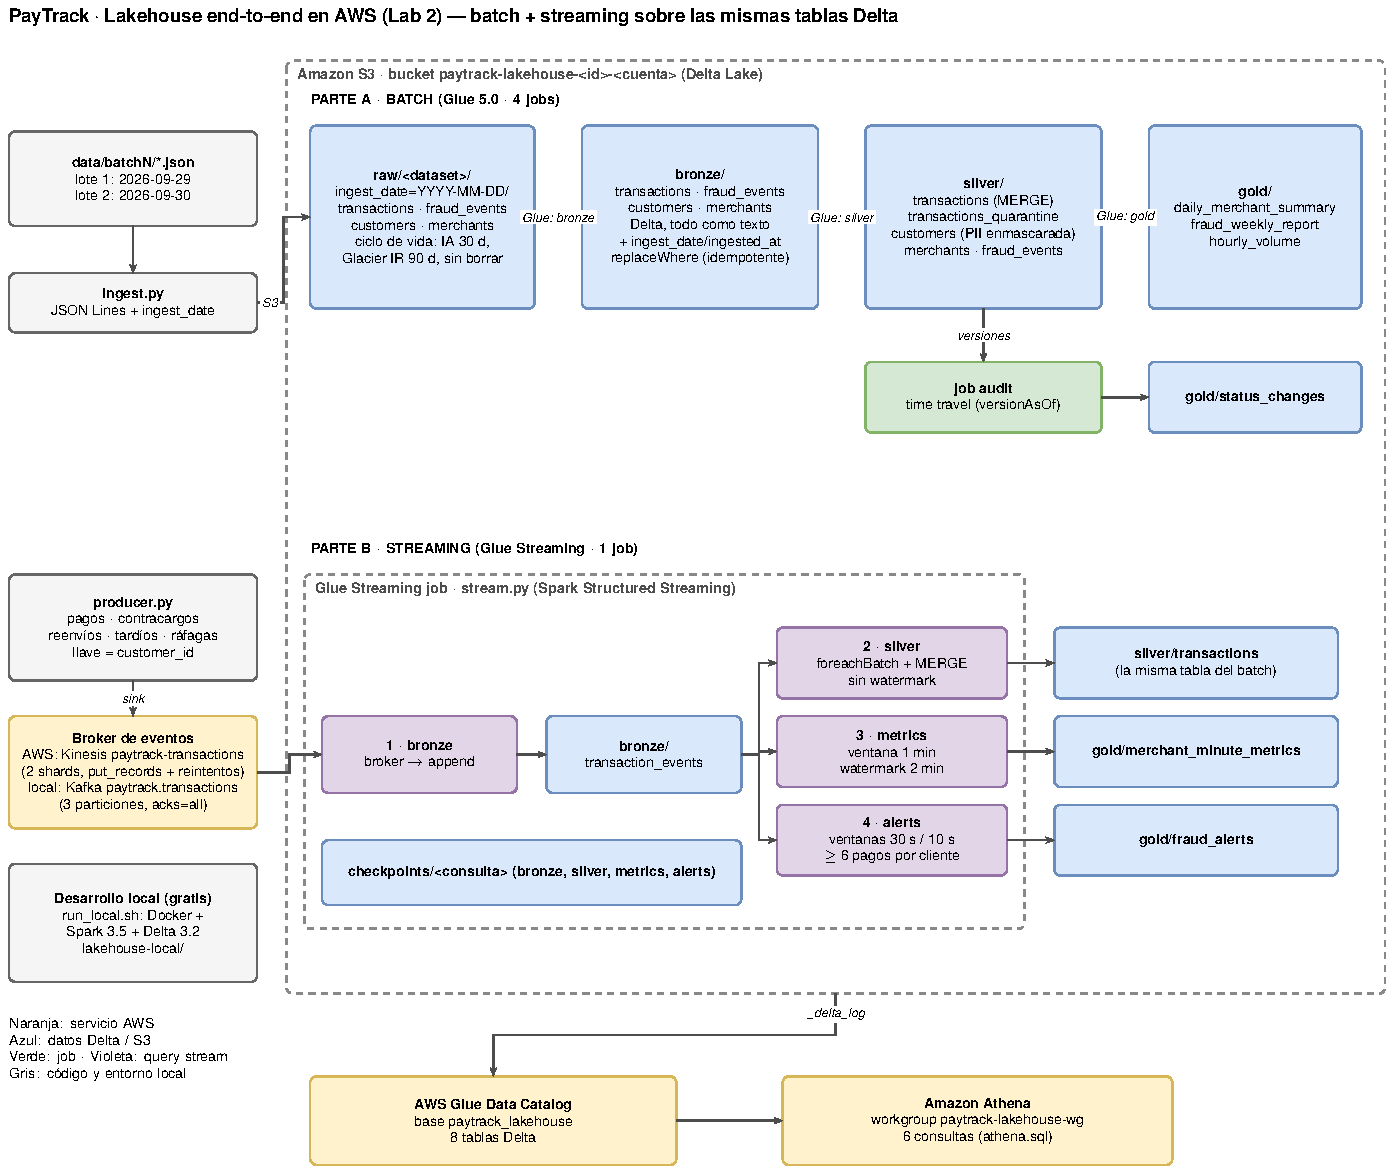
\includegraphics[height=15.2cm]{diagrama/arquitectura.pdf}
\end{landscape}

\section*{Anexo B · Evidencia de AWS (Glue)}
\centering
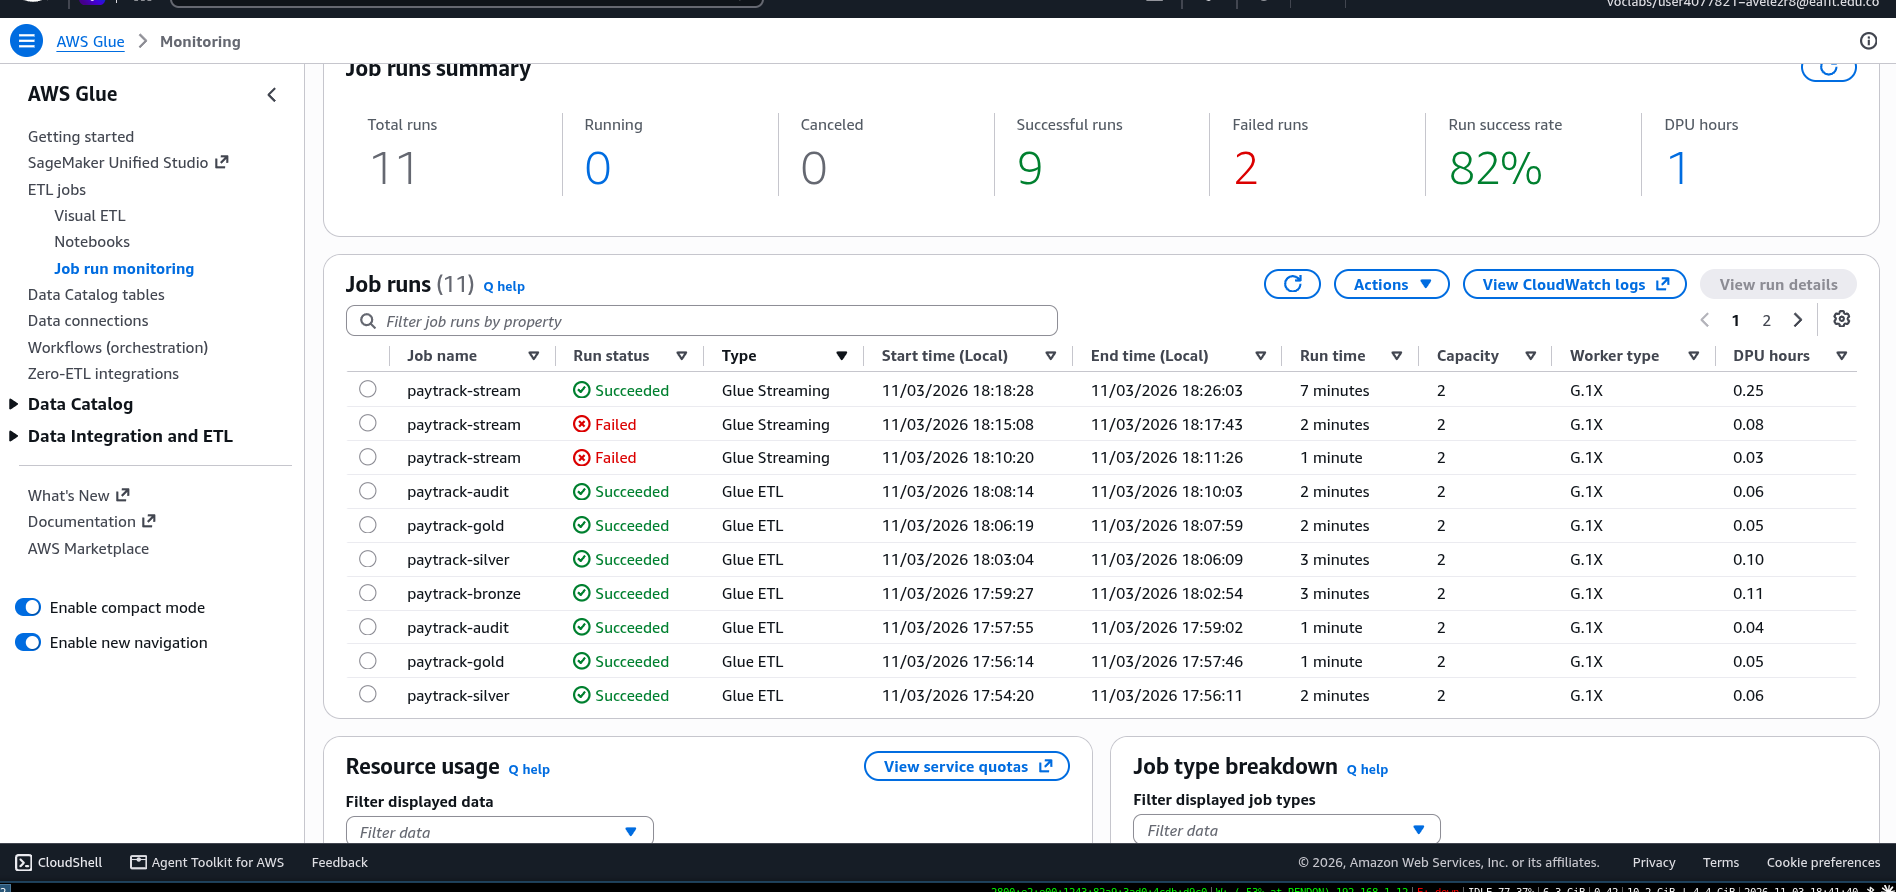
\includegraphics[width=0.92\linewidth]{evidencia/captura_glue_jobs_pag1.png}\\[4pt]
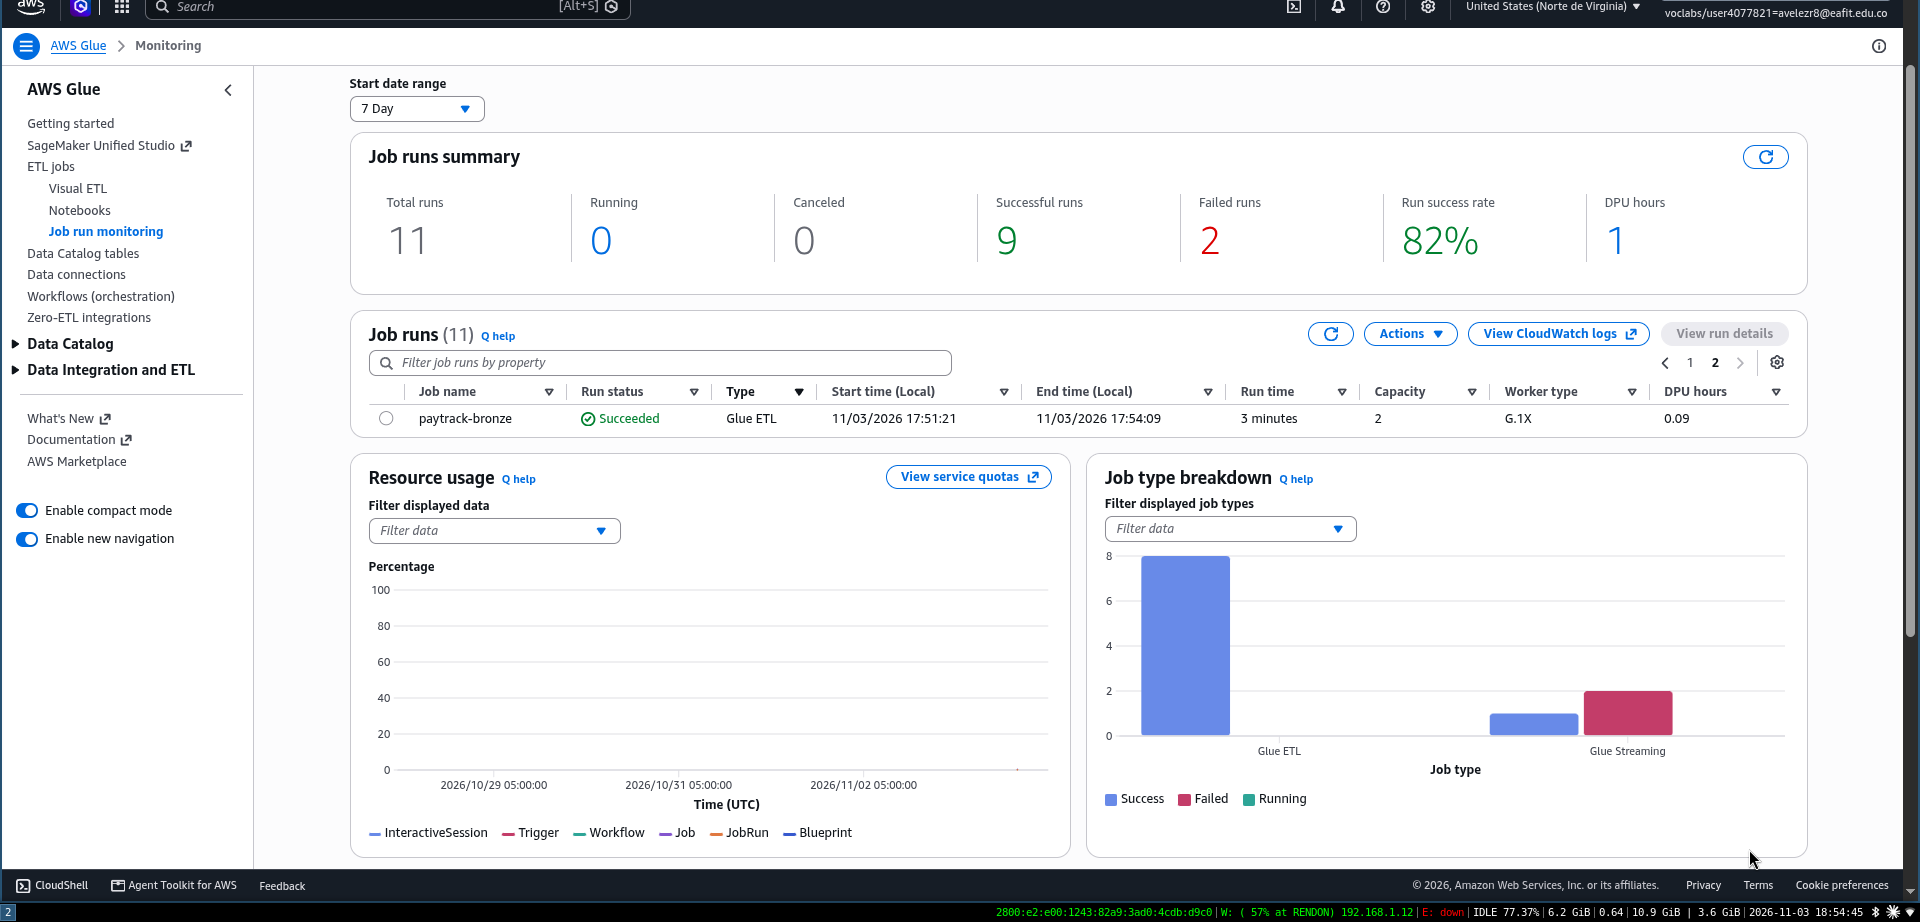
\includegraphics[width=0.92\linewidth]{evidencia/captura_glue_jobs_pag2.png}\\[2pt]
{\small Job run monitoring de Glue: 11 ejecuciones (4 jobs batch $\times$ 2 lotes + 3 del stream: 2 \emph{Failed} previas al arreglo del conector y 1 \emph{Succeeded}). Capturas de las 6 consultas de Athena en \code{informe/evidencia/}.}
\end{document}
